% L7a lecture companion. Notebook hashes and coverage are recorded in README.md.
% Style files and Cornell seal are copied unchanged from the L6c deck, which
% matches the approved L6a deck. The covariance figure is the light PDF from
% ../figs, copied into assets/ by `make figures`.
\documentclass[aspectratio=169,11pt]{beamer}
\usepackage{vnslides}
\usepackage{tabularx}
\renewcommand{\vnlecturecode}{L7a}
\newcolumntype{Y}{>{\raggedright\arraybackslash}X}
\newcommand{\lecturelink}{https://github.com/varnerlab/CHEME-5800-CourseRepository-Fall-2026/blob/main/weeks/week-07/L7a/CHEME-5800-L7a-Lecture-SVDAndDataReduction-Fall-2026.ipynb}
\newcommand{\examplelink}{https://github.com/varnerlab/CHEME-5800-CourseRepository-Fall-2026/blob/main/weeks/week-07/L7a/CHEME-5800-L7a-Example-FunWithSVD-Fall-2026.ipynb}
\newcommand{\lablink}{https://github.com/varnerlab/CHEME-5800-CourseRepository-Fall-2026/blob/main/weeks/week-07/L7b/CHEME-5800-L7b-Lab-SVD-StoichiometricMatrix-Fall-2026.ipynb}
\newcommand{\lecturesource}[1]{\note{[Sources]\par
  \href{\lecturelink}{L7a lecture: Dimensionality Reduction.}\par
  #1\par[/Sources]}}
\newcommand{\Sigmahat}{\hat{\symbf{\Sigma}}}

\title{\texorpdfstring{{\vnheavy L7a}}{L7a}: Dimensionality Reduction}
\subtitle{\texorpdfstring{Covariance, singular value decomposition, and low-rank approximation\\[3pt]CHEME 5800 Cornell University}{Covariance, singular value decomposition, and low-rank approximation; CHEME 5800 Cornell University}}
\author{Copyright Jeffrey Varner 2026. All Rights Reserved}

\begin{document}
\special{pdf:minorversion 7}
\vntitlepage

\begin{frame}{Objectives for Today}
  How can we compress high-dimensional data while keeping its most
  important structure?

  \vspace{0.4em}
  {\large\textbf{\ink{Today's concepts}}}
  \vspace{0.2em}
  \begin{itemize}\setlength{\itemsep}{0.55em}
    \item \hilite{Compute and interpret the empirical covariance matrix}: its
      eigenvectors are the directions of greatest variation, and its eigenvalues
      are the variance along them.
    \item \hilite{Factor a matrix with the singular value decomposition}: compare
      its full, compact, and thin forms, and truncate it for the closest
      lower-rank matrix.
    \item \hilite{Connect principal component analysis to the SVD}: get the same
      directions and variances from the SVD of the centered data.
  \end{itemize}
  \slidenote{Lecture:}{\href{\lecturelink}{Dimensionality Reduction}}
  \lecturesource{Introduction and three Learning Objectives.}
\end{frame}

\begin{frame}{Lecture and Example}
  \textbf{\ink{Lecture:}}
  \href{\lecturelink}{Dimensionality Reduction}

  In this lecture, we build the empirical covariance matrix and its
  eigendecomposition, then factor any matrix with the singular value
  decomposition and truncate it.

  \vspace{1.1em}
  \textbf{\ink{Example:}}
  \href{\examplelink}{Fun with Singular Value Decomposition}

  In this example, we decompose a grayscale photograph into rank-one frames,
  measure how close the first few frames come to the original, and check the
  rank of their sum.

  \vspace{0.8em}
  Dimensionality reduction compresses high-dimensional data while preserving
  its most important structure and information.
  \lecturesource{Introduction and Examples.}
\end{frame}

\begin{frame}{Dimensionality Reduction Problem}
  Suppose we have a dataset of $n$ samples,
  $\mathcal D=\{\mathbf x_1,\mathbf x_2,\ldots,\mathbf x_n\}$, where each
  $\mathbf x_i\in\mathbb R^m$ is an $m$-dimensional feature vector.
  We want to compress each sample into $k$ dimensions:
  \[
    \mathbf x_i\in\mathbb R^m\;\longrightarrow\;\mathbf y_i\in\mathbb R^k,
    \qquad k\ll m.
  \]

  \vspace{0.6em}
  The compressed vectors should keep the most important structure and
  information in the data.

  \vspace{0.6em}
  High-dimensional data is everywhere in modern machine learning, from
  genomics datasets with thousands of features to images with millions of pixels.
  \lecturesource{Introduction and Dimensionality Reduction Problem: dataset and compression map.}
\end{frame}

\begin{frame}{Why Does Dimensionality Reduction Matter?}
  \renewcommand{\arraystretch}{1.2}
  \setlength{\tabcolsep}{5pt}
  \begin{tabularx}{\textwidth}{@{}lY@{}}
    \toprule
    Application & What the reduced representation captures\\
    \midrule
    Genomics & Expression data can have over 20,000 genes but only hundreds of samples; a few key patterns reveal biological processes.\\
    Image compression & A one-megapixel grayscale image has about a million dimensions, but most of its information sits in far fewer components.\\
    Recommendations & Low-dimensional representations of large, sparse user–item matrices capture latent preferences. The Netflix Prize winners used matrix factorization, a close relative of the truncated SVD (\href{https://doi.org/10.1109/MC.2009.263}{Koren et al., 2009}).\\
    Visualization & We cannot plot 1000-dimensional data, but we can plot the top two or three components to spot patterns and clusters.\\
    \bottomrule
  \end{tabularx}
  \lecturesource{Dimensionality Reduction Problem: Why does this matter? callout.}
\end{frame}

\begin{frame}{Composite Features}
  Each entry of the lower-dimensional vector $\mathbf y_i$ is a
  \hilite{composite feature}: a linear combination of the original features
  after subtracting their means.

  \vspace{0.6em}
  Reducing the dimension lets us:
  \begin{itemize}\setlength{\itemsep}{0.55em}
    \item visualize high-dimensional data in two or three dimensions,
    \item reduce the computational cost of a machine learning algorithm, and
    \item store a compact representation that keeps the most important information.
  \end{itemize}

  \vspace{0.6em}
  Which linear combinations keep the most information? We answer this
  question with a linear transformation of the centered data.
  \lecturesource{Dimensionality Reduction Problem: composite features and the benefits of reducing dimensionality.}
\end{frame}

\begin{frame}{A Linear Transformation}
  Suppose a transformation matrix $\mathbf P\in\mathbb R^{k\times m}$ maps
  each sample to its composite features:
  \[
    \mathbf y=\mathbf P\,(\mathbf x-\bar{\mathbf x}),
    \qquad
    y_j=\symbf{\phi}_j^\top(\mathbf x-\bar{\mathbf x}),\quad j=1,2,\ldots,k,
  \]
  where $\bar{\mathbf x}$ is the mean of the feature vectors in the dataset and
  $\symbf{\phi}_j^\top$ is row $j$ of $\mathbf P$. Each row extracts one component.

  \vspace{0.6em}
  What are these transformation vectors $\symbf{\phi}_j$?
  \begin{itemize}\setlength{\itemsep}{0.6em}
    \item They are the top-$k$ eigenvectors of the data's covariance matrix.
      This procedure is \hilite{principal component analysis (PCA)}.
    \item Equivalently, they are the first $k$ right singular vectors of the
      centered data matrix, computed with the \hilite{singular value decomposition (SVD)}.
  \end{itemize}

  \vspace{0.5em}
  The covariance matrix tells us which directions capture the most variance,
  so we review it first.
  \lecturesource{Dimensionality Reduction Problem: transformation matrix, TL;DR (PCA), and the alternative SVD story.}
\end{frame}

\begin{frame}{Sign and Scale of Covariance}
  \centering
  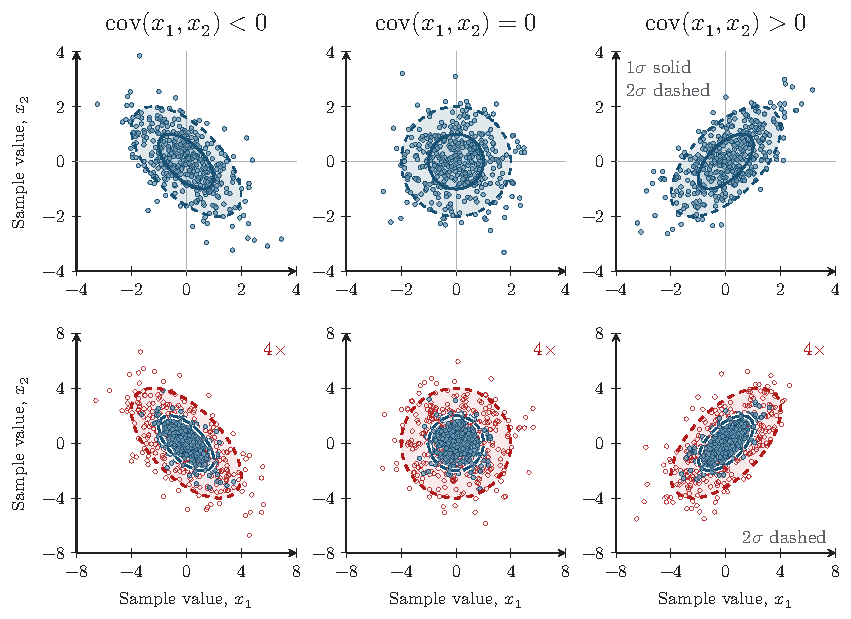
\includegraphics[width=\textwidth,height=0.60\paperheight,keepaspectratio]{assets/Fig-Covariance-Schematic.pdf}

  \vspace{0.4em}
  \raggedright
  The tilt of each ellipse shows the \hilite{sign} of the covariance.
  Multiplying the covariance matrix by four doubles the standard deviations
  and leaves the correlation unchanged.
  \lecturesource{Covariance figure and caption (Sign and scale of covariance).
    Figure: ../figs/Fig-Covariance-Schematic, built in the CHEME 5660 repository
    (lectures/week-5/L5b/figs, commit c4c8710).}
\end{frame}

\begin{frame}{Empirical Covariance Matrix}
  Suppose we have $n$ samples of $m$ features, and let $x_k^{(i)}$ be feature
  $i$ of sample $k$. The \hilite{empirical covariance matrix}
  $\Sigmahat\in\mathbb R^{m\times m}$ is a square symmetric matrix that
  summarizes the covariances between pairs of features. Its entries are:
  \[
    \hat\Sigma_{ij}=\frac{1}{n-1}\sum_{k=1}^{n}
      \bigl(x_k^{(i)}-\bar x_i\bigr)\bigl(x_k^{(j)}-\bar x_j\bigr)
    \quad\Longrightarrow\quad
    \boxed{\hat\Sigma_{ij}=\sigma_i\,\sigma_j\,\rho_{ij}}
  \]
  where $\bar x_i$ is the mean of feature $i$ over the $n$ samples,
  $\sigma_i=\sqrt{\hat\Sigma_{ii}}$ is its standard deviation, and
  $\rho_{ij}\in[-1,1]$ is the correlation between features $i$ and $j$.

  \vspace{0.6em}
  The covariance combines the spread of each feature with how strongly the
  two features move together.
  \lecturesource{Empirical Covariance Matrix: definition, entrywise formula, and boxed result.}
\end{frame}

\begin{frame}{Standard Deviation and Correlation}
  Each diagonal entry of $\Sigmahat$ is the variance of one feature:
  \[
    \sigma_i^2=\hat\Sigma_{ii}
      =\frac{1}{n-1}\sum_{k=1}^{n}\bigl(x_k^{(i)}-\bar x_i\bigr)^2.
  \]
  The correlation divides the covariance by both standard deviations:
  \[
    \rho_{ij}=\frac{\hat\Sigma_{ij}}{\sigma_i\,\sigma_j}
    \quad\Longrightarrow\quad
    \hat\Sigma_{ij}=\sigma_i\,\sigma_j\,\rho_{ij}.
  \]

  \vspace{0.4em}
  The correlation measures the direction and strength of the linear
  relationship on a scale from $-1$ to $1$. In the lower row of the figure,
  scaling the covariance matrix by four doubles each standard deviation and
  leaves the correlation unchanged.
  \lecturesource{Empirical Covariance Matrix: derivation of the boxed result from the variances and the correlation.}
\end{frame}

\begin{frame}{Covariance from the Data Matrix}
  Stack the samples as the rows of the data matrix
  $\mathbf X\in\mathbb R^{n\times m}$, so rows are samples and columns are
  features. Let $\mathbf m=[\bar x_1,\ldots,\bar x_m]^\top$ hold the feature
  means and let $\mathbf 1\in\mathbb R^n$ be a vector of ones.
  The centered data matrix is:
  \[
    \tilde{\mathbf X}=\mathbf X-\mathbf 1\mathbf m^\top.
  \]
  The \hilite{outer product} $\mathbf 1\mathbf m^\top$ is an $n\times m$
  matrix whose rows all equal $\mathbf m^\top$. In general, the outer product
  of $\mathbf a\in\mathbb R^n$ and $\mathbf b\in\mathbb R^m$ has entries
  $(\mathbf a\mathbf b^\top)_{ij}=a_i b_j$. The empirical covariance matrix is then:
  \[
    \Sigmahat=\frac{1}{n-1}\,\tilde{\mathbf X}^\top\tilde{\mathbf X}.
  \]
  This form computes every covariance at once.
  \lecturesource{Empirical Covariance Matrix: data matrix, centering, outer-product callout, and matrix form.}
\end{frame}

\begin{frame}{Covariance Matrix Properties}
  \begin{itemize}\setlength{\itemsep}{0.75em}
    \item \hilite{Elements}: the diagonal entries $\hat\Sigma_{ii}$ are the
      variances of the features and are never negative. The off-diagonal
      entries $\hat\Sigma_{ij}$, $i\ne j$, are the covariances between pairs of features.
    \item \hilite{Sign}: if $\hat\Sigma_{ij}>0$, feature $j$ tends to be above
      its mean when feature $i$ is above its mean. If $\hat\Sigma_{ij}<0$,
      feature $j$ tends to be below its mean when feature $i$ is above its mean. If $\hat\Sigma_{ij}=0$, the features are uncorrelated:
      there is no linear relationship between them.
    \item \hilite{Symmetry}: $\hat\Sigma_{ij}=\hat\Sigma_{ji}$ for all $i$ and
      $j$, which follows from the definition of covariance.
    \item \hilite{Positive semidefinite}: $\mathbf v^\top\Sigmahat\,\mathbf v
      =\frac{1}{n-1}\|\tilde{\mathbf X}\mathbf v\|_2^2\ge0$ for every vector
      $\mathbf v\in\mathbb R^m$, since it is the variance of the centered data
      projected onto $\mathbf v$.
  \end{itemize}
  \lecturesource{Empirical Covariance Matrix: Covariance Matrix Properties callout.}
\end{frame}

\begin{frame}{Decomposing the Covariance Matrix}
  Because $\Sigmahat$ is real, symmetric, and positive semidefinite, its
  eigenpairs $(\mathbf v_i,\lambda_i)$ have special properties. We can write:
  \[
    \Sigmahat=\mathbf V\,\symbf{\Lambda}\,\mathbf V^\top,
    \qquad
    \symbf{\Lambda}=\operatorname{diag}(\lambda_1,\ldots,\lambda_m),
  \]
  where $\mathbf V=[\mathbf v_1,\ldots,\mathbf v_m]\in\mathbb R^{m\times m}$
  holds the eigenvectors as columns.

  \vspace{0.4em}
  \begin{itemize}\setlength{\itemsep}{0.6em}
    \item \hilite{Orthonormal eigenvectors}: the eigenvectors can be chosen as
      mutually orthogonal unit vectors, so $\mathbf V^\top\mathbf V=\mathbf I$,
      the identity matrix.
    \item \hilite{Nonnegative eigenvalues}: the eigenvalues can be ordered as
      $\lambda_1\ge\lambda_2\ge\cdots\ge\lambda_m\ge0$.
    \item Each eigenvalue $\lambda_i$ equals the \hilite{variance of the data}
      along the direction $\mathbf v_i$.
  \end{itemize}
  \lecturesource{Decomposing the Covariance Matrix: properties 1 and 2.}
\end{frame}

\begin{frame}{Principal Components}
  Projecting a sample's deviation from the mean onto $\mathbf v_i$ gives its
  $i$-th \hilite{principal component}:
  \[
    y_i=\mathbf v_i^\top(\mathbf x-\bar{\mathbf x}).
  \]
  Across the dataset, $y_i$ has variance $\lambda_i$. The direction
  $\mathbf v_1$ captures the most variance, the direction $\mathbf v_2$
  captures the second most, and so on.

  \vspace{0.6em}
  Keeping the top $k$ eigenvectors,
  $\mathbf V_k=[\mathbf v_1,\ldots,\mathbf v_k]$, gives the best
  $k$-dimensional linear reconstruction of the data in the least-squares
  sense. The subspace they span \hilite{maximizes the retained variance} and
  \hilite{minimizes the reconstruction error}.

  \vspace{0.6em}
  These eigenpairs are the foundation of PCA: the rows of the transformation
  matrix $\mathbf P$ are $\mathbf v_1^\top,\ldots,\mathbf v_k^\top$.
  \lecturesource{Decomposing the Covariance Matrix: properties 3 and 4 and the closing PCA sentence.}
\end{frame}

\begin{frame}{From Eigendecomposition to SVD}
  The eigendecomposition works for square, symmetric matrices such as
  $\Sigmahat$. The centered data matrix
  $\tilde{\mathbf X}\in\mathbb R^{n\times m}$ is usually rectangular, with more
  samples than features or the reverse.

  \vspace{0.7em}
  The \hilite{singular value decomposition} factors any rectangular matrix.
  Applied to the centered data matrix $\tilde{\mathbf X}$, it gives the same
  principal directions as the eigendecomposition of $\Sigmahat$, so the two
  approaches are mathematically equivalent.

  \vspace{0.7em}
  The SVD has become the workhorse of dimensionality reduction because it is
  more general, it is numerically stable, and it factors the data matrix directly.
  \lecturesource{From Eigendecomposition to SVD: limitation, Enter SVD! callout, and closing sentence.}
\end{frame}

\begin{frame}{Singular Value Decomposition}
  Given any matrix $\mathbf A\in\mathbb R^{m\times n}$ of rank $r=r(\mathbf A)$,
  the \hilite{full SVD} is the factorization:
  \[
    \mathbf A=\mathbf U\,\mathbf S\,\mathbf V^\top.
  \]
  \begin{itemize}\setlength{\itemsep}{0.35em}
    \item $\mathbf U\in\mathbb R^{m\times m}$ is orthogonal,
      $\mathbf U^\top\mathbf U=\mathbf I_m$ (the identity), and its columns
      $\mathbf u_i$ are the \hilite{left singular vectors}.
    \item $\mathbf S\in\mathbb R^{m\times n}$ is rectangular diagonal, with the
      \hilite{singular values} $\sigma_1\ge\cdots\ge\sigma_r>0$ on its first
      $r$ diagonal entries and zeros elsewhere. From here on, $\sigma_i$
      denotes a singular value.
    \item $\mathbf V\in\mathbb R^{n\times n}$ is orthogonal,
      $\mathbf V^\top\mathbf V=\mathbf I_n$ (the identity), and its columns
      $\mathbf v_i$ are the \hilite{right singular vectors}.
  \end{itemize}

  \vspace{0.3em}
  The singular values are the square roots of the eigenvalues of
  $\mathbf A^\top\mathbf A$, so $\sigma_i=\sqrt{\lambda_i(\mathbf A^\top\mathbf A)}$.
  The number of nonzero singular values is the rank of $\mathbf A$, and
  $r(\mathbf A)\le\min(m,n)$.
  \lecturesource{Singular value decomposition: full SVD and its factors.}
\end{frame}

\begin{frame}{Full and Compact SVD}
  The full SVD stores all $m$ left singular vectors and all $n$ right singular
  vectors, even though only the first $r(\mathbf A)$ correspond to nonzero
  singular values.

  \vspace{0.3em}
  \begin{itemize}\setlength{\itemsep}{0.4em}
    \item \hilite{Pro}: the full factors give complete orthonormal bases for
      $\mathbb R^m$ and $\mathbb R^n$; the first $r(\mathbf A)$ columns of
      $\mathbf U$ and $\mathbf V$ span the column and row spaces of $\mathbf A$.
    \item \hilite{Con}: the memory requirement grows as
      $\mathcal O(m^2+n^2)$, which is wasteful when $r(\mathbf A)\ll\min(m,n)$.
  \end{itemize}

  \vspace{0.3em}
  The \hilite{compact SVD} keeps only the first $r=r(\mathbf A)$ singular vectors
  and singular values:
  \[
    \mathbf A=\mathbf U_r\,\mathbf S_r\,\mathbf V_r^\top,
    \qquad
    \mathbf U_r\in\mathbb R^{m\times r},\quad
    \mathbf S_r\in\mathbb R^{r\times r},\quad
    \mathbf V_r\in\mathbb R^{n\times r}.
  \]
  The \hilite{thin SVD} sits in between: it keeps $\min(m,n)$ singular vectors
  on each side. Julia's \texttt{svd(...)} function returns the thin SVD by default.
  \lecturesource{Singular value decomposition: full SVD pros and cons, the compact SVD, and the thin SVD.}
\end{frame}

\begin{frame}{PCA from the SVD}
  Let the centered data matrix $\tilde{\mathbf X}\in\mathbb R^{n\times m}$ have
  the full SVD $\tilde{\mathbf X}=\mathbf U\mathbf S\mathbf V^\top$.
  Substituting into the covariance matrix and using
  $\mathbf U^\top\mathbf U=\mathbf I_n$ gives:
  \[
    \Sigmahat=\frac{1}{n-1}\tilde{\mathbf X}^\top\tilde{\mathbf X}
    =\frac{1}{n-1}\mathbf V\mathbf S^\top
      \underbrace{\mathbf U^\top\mathbf U}_{\mathbf I_n}\mathbf S\mathbf V^\top
    =\mathbf V\left(\frac{\mathbf S^\top\mathbf S}{n-1}\right)\mathbf V^\top.
  \]
  Here $\mathbf S^\top\mathbf S$ is diagonal with entries $\sigma_i^2$, where
  $\sigma_i$ are the singular values of $\tilde{\mathbf X}$. This is the
  eigendecomposition $\Sigmahat=\mathbf V\symbf{\Lambda}\mathbf V^\top$:
  \begin{itemize}\setlength{\itemsep}{0.4em}
    \item the right singular vectors of $\tilde{\mathbf X}$ are the
      \hilite{eigenvectors} of $\Sigmahat$, and
    \item the eigenvalues are $\lambda_i=\sigma_i^2/(n-1)$, taking $\sigma_i=0$ for $i>r(\tilde{\mathbf X})$.
  \end{itemize}

  \vspace{0.4em}
  We can compute the principal directions and their variances from the SVD
  of $\tilde{\mathbf X}$ without forming $\Sigmahat$.
  \lecturesource{Singular value decomposition: PCA from the SVD subsection and callout.}
\end{frame}

\begin{frame}{Dimensionality Reduction with the SVD}
  The SVD writes any rectangular matrix as a weighted sum of rank-one matrices:
  \[
    \mathbf A=\sum_{i=1}^{r(\mathbf A)}\sigma_i\,
      \underbrace{\left(\mathbf u_i\otimes\mathbf v_i\right)}_{\mathbf u_i\mathbf v_i^\top}
  \]
  where $\mathbf u_i$ and $\mathbf v_i$ are the $i$-th left and right singular
  vectors and $\sigma_i$ are the ordered singular values. The outer product
  $\mathbf u_i\mathbf v_i^\top$ is an $m\times n$ matrix of rank one, a
  separable \hilite{rank-one component} of $\mathbf A$.

  \vspace{0.7em}
  The components are weighted by their singular values, largest first.
  Truncating the sum keeps the components with the largest weights, which makes
  the SVD well suited to dimensionality reduction and data compression.
  \lecturesource{Singular value decomposition: Dimensionality Reduction? subsection, sum of rank-one matrices.}
\end{frame}

\begin{frame}{Eckart–Young Theorem}
  Truncate the sum after $k<r(\mathbf A)$ terms:
  \[
    \mathbf A_k=\sum_{i=1}^{k}\sigma_i\,\mathbf u_i\mathbf v_i^\top.
  \]
  For any other matrix $\mathbf B\in\mathbb R^{m\times n}$ of rank at most $k$:
  \[
    \|\mathbf A-\mathbf A_k\|_F\le\|\mathbf A-\mathbf B\|_F,
    \qquad
    \|\mathbf A-\mathbf A_k\|_2\le\|\mathbf A-\mathbf B\|_2,
  \]
  where $\|\cdot\|_F$ is the Frobenius norm and $\|\cdot\|_2$ is the operator
  (spectral) norm.

  \vspace{0.7em}
  Truncating the SVD is \hilite{provably optimal}: $\mathbf A_k$ is the
  closest rank-$k$ matrix to $\mathbf A$, whether we measure closeness by the
  total squared error (the squared Frobenius norm) or by the maximum stretch
  (the spectral norm).
  \lecturesource{Singular value decomposition: Eckart–Young theorem callout and interpretation.}
\end{frame}

\begin{frame}{Example: Fun with Singular Value Decomposition}
  In this example, we decompose a grayscale photograph into rank-one frames
  and rebuild it from the first few.

  \vspace{0.6em}
  \begin{enumerate}\setlength{\itemsep}{0.65em}
    \item Compute the SVD of the image matrix and check that $\mathbf U$ and
      $\mathbf V$ are orthogonal and that the factors multiply back to the image.
    \item Compute the frames and measure the relative error, in the Frobenius
      norm, of the image built from the first $k$ frames.
    \item Add up the first few frames and check that the rank of the sum
      equals the number of frames.
  \end{enumerate}

  \vspace{0.6em}
  The example does not center the image, so the first frame mostly holds the
  image's average brightness. The later frames add edges and finer detail.
  \slidenote{Example:}{\href{\examplelink}{Fun with Singular Value Decomposition}}
  \lecturesource{Singular value decomposition: example callout.
    Companion example: Tasks 1–3 and the explanation after the relative-error plot.}
\end{frame}

\begin{frame}{Lab: SVD of a Platelet Metabolic Network}
  In \href{\lablink}{L7b}, we construct a stoichiometric matrix from a human
  platelet metabolic model and use its SVD to examine:

  \vspace{0.6em}
  \begin{itemize}\setlength{\itemsep}{0.7em}
    \item the \hilite{numerical rank} of the stoichiometric matrix,
    \item \hilite{matrix reconstruction} from the leading modes, and
    \item \hilite{conservation relations} and \hilite{balanced-flux directions}.
  \end{itemize}

  \vspace{0.7em}
  The same decomposition that compresses an image also reveals the structure
  of a reaction network.
  \slidenote{Lab:}{\href{\lablink}{SVD of a platelet stoichiometric matrix}}
  \lecturesource{Lab section.}
\end{frame}

\begin{frame}{Summary}
  We used matrix decompositions to find the most important directions in
  high-dimensional data.

  \vspace{0.6em}
  {\large\textbf{\ink{Key takeaways}}}
  \vspace{0.3em}
  \begin{itemize}\setlength{\itemsep}{0.9em}
    \item \textbf{\ink{Covariance eigendecomposition.}} The eigenvectors are the
      principal directions; the eigenvalues are the variance along each one.
    \item \textbf{\ink{Truncated SVD.}} Keeping the largest singular values gives
      the closest matrix of that rank in the Frobenius and spectral norms.
    \item \textbf{\ink{PCA from the SVD.}} The SVD of the centered data gives the
      principal directions and variances without forming the covariance matrix.
  \end{itemize}

  \vspace{0.8em}
  The example and lab apply these ideas to an image and a metabolic network.
  \lecturesource{Summary: three key takeaways and concluding sentence.}
\end{frame}

\end{document}
